\documentclass[a4paper,12px]{article}
\usepackage{graphicx}
\usepackage[english]{babel}
\usepackage{fancyhdr}
\usepackage{lastpage}
\usepackage{xifthen}
\usepackage[linesnumberedhidden, titlenotnumbered]{algorithm2e}
\usepackage{lipsum}
\usepackage{hyperref}
\usepackage{array}
\usepackage{tabularx}

\usepackage{minted}
\usepackage{caption}
\usepackage{amssymb}

\pagestyle{fancy}
\lhead{
\includegraphics[width=7cm]{logoUvA}}
\rhead{\footnotesize \textsc {Report\\ \opdracht}}
\lfoot
{
    \footnotesize \studentA
    \ifthenelse{\isundefined{\studentB}}{}{\\ \studentB}
    \ifthenelse{\isundefined{\studentC}}{}{\\ \studentC}
    \ifthenelse{\isundefined{\studentD}}{}{\\ \studentD}
    \ifthenelse{\isundefined{\studentE}}{}{\\ \studentE}
}
\cfoot{}
\rfoot{\small \textsc {Page \thepage\ of \pageref{LastPage}}}
\renewcommand{\footrulewidth}{0.5pt}

\fancypagestyle{firststyle}
{
    \fancyhf{}
    \renewcommand{\headrulewidth}{0pt}
    \chead{
\includegraphics[width=7cm]{logoUvA}}
    \rfoot{\small \textsc {Page \thepage\ of \pageref{LastPage}}}
}

\setlength{\topmargin}{-0.3in}
\setlength{\textheight}{630pt}
\setlength{\headsep}{40pt}

% =================================== DOC INFO ===================================

\newcommand{\titel}{OpenMP}
\newcommand{\opdracht}{Assignment 2.1: Wave}
\newcommand{\docent}{Dr. C. Grelck}
\newcommand{\cursus}{Concurrency and Parallel Programming}
\newcommand{\vakcode}{5062COPP6Y}
\newcommand{\datum}{\today}
\newcommand{\studentA}{Robin Klusman}
\newcommand{\uvanetidA}{10675671}
\newcommand{\studentB}{Maico Timmerman}
\newcommand{\uvanetidB}{10542590}
%\newcommand{\studentC}{Boudewijn Braams}
\newcommand{\uvanetidC}{10401040}
%\newcommand{\studentD}{Govert Verkes}
\newcommand{\uvanetidD}{10211748}
%\newcommand{\studentE}{Naam student 5}
\newcommand{\uvanetidE}{UvAnetID student 5}

% ===================================  ===================================

\begin{document}
\thispagestyle{firststyle}
\begin{center}
    \textsc{\Large \opdracht}\\[0.2cm]
    \rule{\linewidth}{0.5pt} \\[0.4cm]
    {\huge \bfseries \titel}
    \rule{\linewidth}{0.5pt} \\[0.2cm]
    {\large \datum  \\[0.4cm]}

    \begin{minipage}{0.4\textwidth}
        \begin{flushleft}
            \emph{Student:}\\
            {\studentA \\ {\small \uvanetidA \\[0.2cm]}}
            \ifthenelse{\isundefined{\studentB}}{}{\studentB \\ {\small \uvanetidB \\[0.2cm]}}
            \ifthenelse{\isundefined{\studentC}}{}{\studentC \\ {\small \uvanetidC \\[0.2cm]}}
            \ifthenelse{\isundefined{\studentD}}{}{\studentD \\ {\small \uvanetidD \\[0.2cm]}}
            \ifthenelse{\isundefined{\studentE}}{}{\studentE \\ {\small \uvanetidE \\ [0.2cm]}}
        \end{flushleft}
    \end{minipage}
    ~
    \begin{minipage}{0.4\textwidth}
        \begin{flushright}
            \emph{Supervisor:} \\
            \docent \\[0.2cm]
            \emph{Course:} \\
            \cursus \\[0.2cm]
            \emph{Course code:} \\
            \vakcode \\[0.2cm]
        \end{flushright}
    \end{minipage}\\[1 cm]
\end{center}


% =================================== FRONT PAGE ===================================

\vspace{2cm}
\begin{center}
    
\includegraphics[width=(\textwidth/5*3)]{parallel_tasks}
\end{center}
\clearpage

\tableofcontents
\vspace{5mm}

% =================================== MAIN TEXT ===================================

\section{Introduction}

In this assignment we take another look at the wave equation simulation, now
with a different kind of parallel programming. This time OpenMP is used to make
our code concurrent. OpenMP works by the programmer stating some part of the
code can be run in parallel (in this case a for-loop) and then the compiler will
compile the code so that it is concurrent.

\section{Method}

Implementing OpenMP is quite simple, all that needed to be done was to write a
sequential program for the wave equation simulation, and then state that a
certain for-loop can be done in parallel using the OpenMP commands. There are
however several different ways of scheduling that can be used when parallelizing
a for-loop with openMP and we will test all of them to see which is the most
effective. Those results will then again be compared to the results we found
with our results from the previous assignment using pthreads to parallelize this
program.

\section{Results}

Running the new Wave Simulation that implements OpenMP on the DAS4 machine we
found some minor differences in the time the simulation takes to complete.
Running it with only one thread, a clear difference can be seen between the
OpenMP implementation and the pthread implementation, especially when using
static scheduling. When using dynamic or guided scheduling we see a less
significant difference running it with a single thread, but a more difference
when running with more than one thread.

\begin{figure}[H]
    \centering
    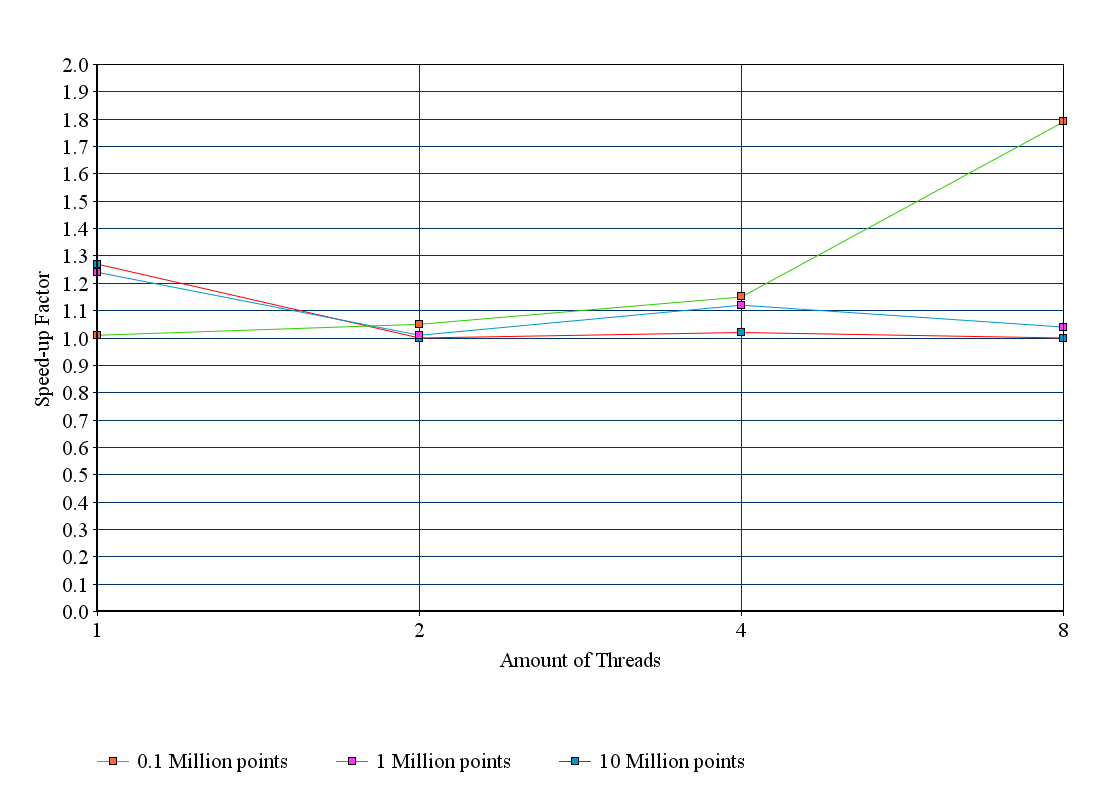
\includegraphics[width=\textwidth]{static}
    \caption{Speed-up factor of using OpenMP static scheduling compared to the
    same amount of threads and amplitude points using the pthread approach. Runs
    a total of 10000 time steps over different amounts of amplitude points.}
\end{figure}

\begin{figure}[H]
    \centering
    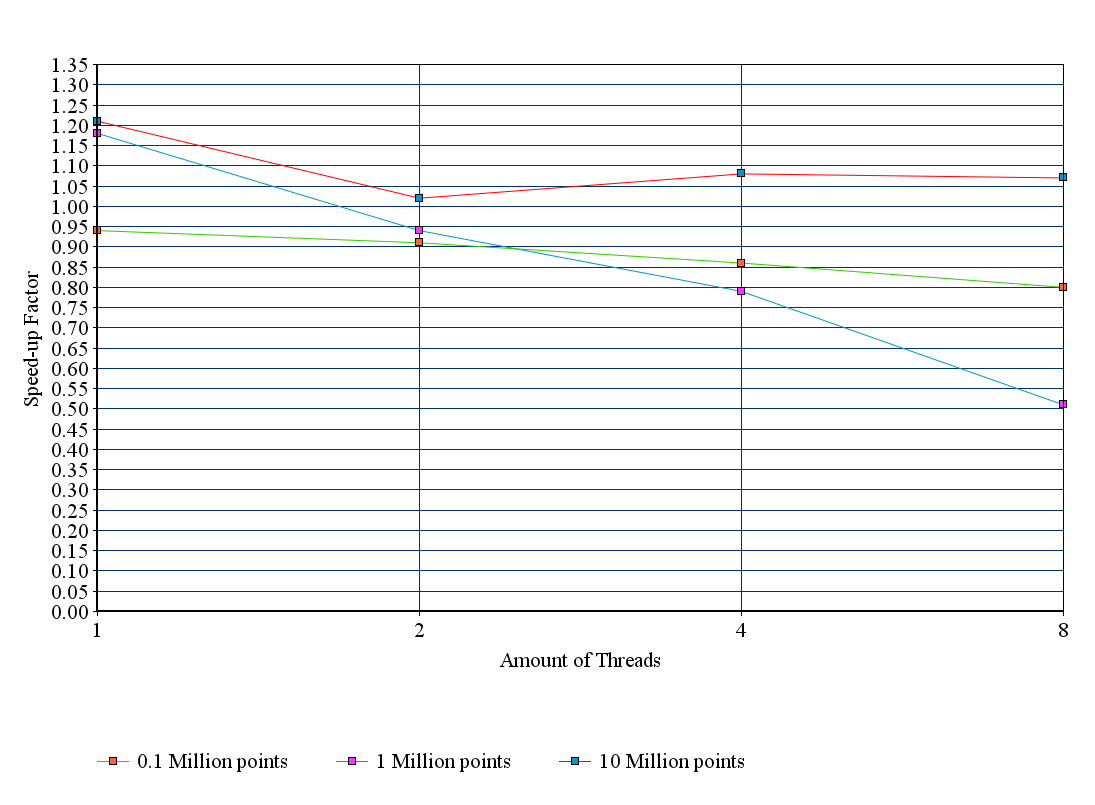
\includegraphics[width=\textwidth]{dynamic}
    \caption{Speed-up factor of using OpenMP dynamic scheduling compared to the
    same amount of threads and amplitude points using the pthread approach. Runs
    a total of 10000 time steps over different amounts of amplitude points.}
\end{figure}

\begin{figure}[H]
    \centering
    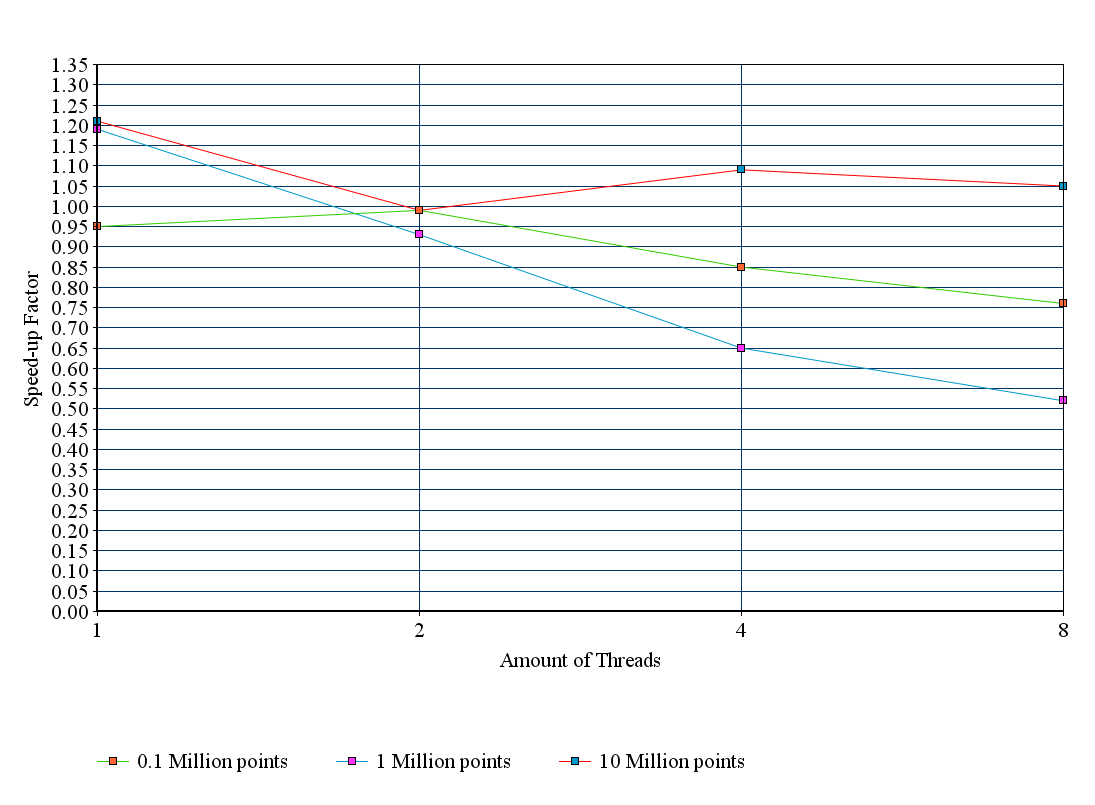
\includegraphics[width=\textwidth]{guided}
    \caption{Speed-up factor of using OpenMP guided scheduling compared to the
    same amount of threads and amplitude points using the pthread approach. Runs
    a total of 10000 time steps over different amounts of amplitude points.}
\end{figure}

\section{Discussion}
A clear speed-up is seen when comparing the pthread program run with a single
thread to the OpenMP version. This can be explained by the overhead created in
the pthread program from synchronising and mutex locking (which in the case of 1
thread does not even need to be done). OpenMP seemingly does not create all this
overhead when running with a single thread, because it is not needed.\\
In addition to this quite irrelevant speed-up that only occurs when running with
one thread, a slight decrease of the runtime is also evident when running ten
million points on eight cores. This indicates that OpenMP is more efficient at
writing concurrent code than we were when we made the last assignment, which is
not very hard to believe. \\
The differences between the dynamic, guided and static scheduling modes of
OpenMP can be explained by their complexity. Dynamic and guided scheduling are
in theory better than static, but the static version outperforms them both when
running with a single thread. This is most likely due to the more complex nature
of guided and dynamic scheduling, which creates a little more overhead and does
not yield any speed-up when using only one thread.


% =================================== REFERENCES ===================================

%\clearpage
%\bibliographystyle{unsrt}
%\bibliography{bib}

\end{document}
